\section{Previous Work}
Some Research has been done before, the study of this thesis comes after some seniors' effort. For example, Ryo Kita's research ``Matching Legal Aspects with Cases based on Descriptive Similarities'' and Zhang Xiaolong's research ``Towards a Detection of Descriptive Similarities among Multiple Precedents Based on Formal Concept Analysis''. Some important points are used for reference such as the using of KNP tool, the similarity between noun-object similarity classes, using the database of legal precedents, etc. There are still very different points between the seniors' research and this research.
In Ryo Kita's research, the event is a verb and noun pair, think of the matching as a transmission problem the matching is one on one between the abstract and main text of a precedent.[12]\\
In Zhang Xiaolong's research, the event is defined as a list of the verb and noun pairs, this point is the same as this thesis. In his research, he regards the events of each precedent as a concrete graph, and try to find the similar structure of the concrete graphs and build the similar structure as an abstract graph. He also only concerns the matching between two documents.[13]\\
\begin{figure}[!hbp]
\centering
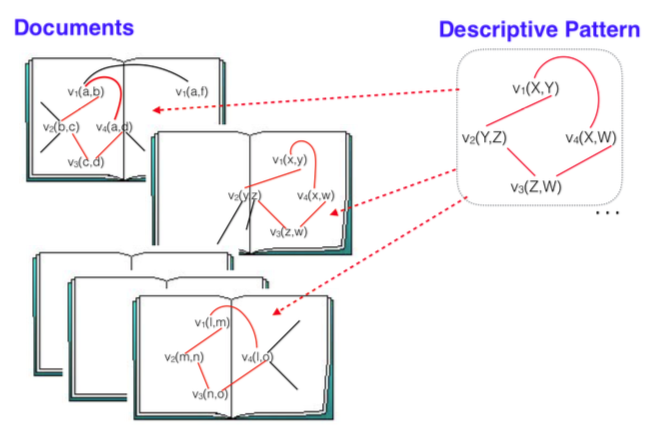
\includegraphics[width=300pt]{./pictures/0103.png}
\caption{Zhang's research}
\end{figure}
Both of them uses the importance of noun defined by the KeyGraph algorithm, but they didn't verify the result of KeyGraph, how the High KeyScore nouns influence the result of similarity classes, we will use some sections to talk about the result of KeyGraph, and whether is it safe to disregard nouns which are not high KeyScore nouns.\\
Besides, we don't concern the event graphs, we proposed a method to extract descriptive patterns from maximal closures.\\
We have three new points to experiment as they are very important points:
\begin{enumerate}
\item We don't use the idea of the concrete graph and abstract graph, although they exist as a fact, we use a more direct way to extract descriptive patterns.
\item We concern more than two documents, the problem will be not a matching problem, it becomes a kind of data mining problem.
\item We will verify the feasibility of KeyGrpah, and talk about the result of it.
\end{enumerate}